\documentclass[a4paper, 14pt]{extarticle}

% Поля
%--------------------------------------
\usepackage{geometry}
\geometry{a4paper,tmargin=2cm,bmargin=2cm,lmargin=3cm,rmargin=1cm}
%--------------------------------------


%Russian-specific packages
%--------------------------------------
\usepackage[T2A]{fontenc}
\usepackage[utf8]{inputenc}
\usepackage[english, main=russian]{babel}
%--------------------------------------

\usepackage{textcomp}

% Красная строка
%--------------------------------------
\usepackage{indentfirst}
%--------------------------------------


%Graphics
%--------------------------------------
\usepackage{graphicx}
\graphicspath{ {./images/} }
\usepackage{wrapfig}
%--------------------------------------

% Полуторный интервал
%--------------------------------------
\linespread{1.3}
%--------------------------------------

%Выравнивание и переносы
%--------------------------------------
% Избавляемся от переполнений
\sloppy
% Запрещаем разрыв страницы после первой строки абзаца
\clubpenalty=10000
% Запрещаем разрыв страницы после последней строки абзаца
\widowpenalty=10000
%--------------------------------------

%Списки
\usepackage{enumitem}

%Подписи
\usepackage{caption}

%Гиперссылки
\usepackage{hyperref}

\hypersetup {
	unicode=true
}

%Рисунки
%--------------------------------------
\DeclareCaptionLabelSeparator*{emdash}{~--- }
\captionsetup[figure]{labelsep=emdash,font=onehalfspacing,position=bottom}
%--------------------------------------

\usepackage{tempora}

%Листинги
%--------------------------------------
\usepackage{listings}
\lstset{
  basicstyle=\ttfamily\footnotesize,
  %basicstyle=\footnotesize\AnkaCoder,        % the size of the fonts that are used for the code
  breakatwhitespace=false,         % sets if automatic breaks shoulbd only happen at whitespace
  breaklines=true,                 % sets automatic line breaking
  captionpos=t,                    % sets the caption-position to bottom
  inputencoding=utf8,
  frame=single,                    % adds a frame around the code
  keepspaces=true,                 % keeps spaces in text, useful for keeping indentation of code (possibly needs columns=flexible)
  keywordstyle=\bf,       % keyword style
  numbers=left,                    % where to put the line-numbers; possible values are (none, left, right)
  numbersep=5pt,                   % how far the line-numbers are from the code
  xleftmargin=25pt,
  xrightmargin=25pt,
  showspaces=false,                % show spaces everywhere adding particular underscores; it overrides 'showstringspaces'
  showstringspaces=false,          % underline spaces within strings only
  showtabs=false,                  % show tabs within strings adding particular underscores
  stepnumber=1,                    % the step between two line-numbers. If it's 1, each line will be numbered
  tabsize=2,                       % sets default tabsize to 8 spaces
  title=\lstname                   % show the filename of files included with \lstinputlisting; also try caption instead of title
}
%--------------------------------------

%%% Математические пакеты %%%
%--------------------------------------
\usepackage{amsthm,amsfonts,amsmath,amssymb,amscd}  % Математические дополнения от AMS
\usepackage{mathtools}                              % Добавляет окружение multlined
\usepackage[perpage]{footmisc}
%--------------------------------------

%--------------------------------------
%			НАЧАЛО ДОКУМЕНТА
%--------------------------------------

\begin{document}

%--------------------------------------
%			ТИТУЛЬНЫЙ ЛИСТ
%--------------------------------------
\begin{titlepage}
\thispagestyle{empty}
\newpage


%Шапка титульного листа
%--------------------------------------
\vspace*{-60pt}
\hspace{-65pt}
\begin{minipage}{0.3\textwidth}
\hspace*{-20pt}\centering

\includegraphics[width=\textwidth]{emblem}
\end{minipage}
\begin{minipage}{0.67\textwidth}\small \textbf{
\vspace*{-0.7ex}
\hspace*{-6pt}\centerline{Министерство науки и высшего образования Российской Федерации}
\vspace*{-0.7ex}
\centerline{Федеральное государственное бюджетное образовательное учреждение }
\vspace*{-0.7ex}
\centerline{высшего образования}
\vspace*{-0.7ex}
\centerline{<<Московский государственный технический университет}
\vspace*{-0.7ex}
\centerline{имени Н.Э. Баумана}
\vspace*{-0.7ex}
\centerline{(национальный исследовательский университет)>>}
\vspace*{-0.7ex}
\centerline{(МГТУ им. Н.Э. Баумана)}}
\end{minipage}
%--------------------------------------

%Полосы
%--------------------------------------
\vspace{-25pt}
\hspace{-35pt}\rule{\textwidth}{2.3pt}

\vspace*{-20.3pt}
\hspace{-35pt}\rule{\textwidth}{0.4pt}
%--------------------------------------

\vspace{1.5ex}
\hspace{-35pt} \noindent \small ФАКУЛЬТЕТ\hspace{30pt} <<Информатика, искусственный интеллект и системы управления>>

\vspace*{-16pt}
\hspace{47pt}\rule{0.83\textwidth}{0.4pt}

\vspace{0.5ex}
\hspace{-35pt} \noindent \small КАФЕДРА\hspace{50pt} <<Теоретическая информатика и компьютерные технологии>>

\vspace*{-16pt}
\hspace{30pt}\rule{0.866\textwidth}{0.4pt}

\vspace{11em}

\begin{center}
\Large {\bf Летучка  № 2} \\
\large {\bf по курсу <<Языки и методы программирования>>} \\
\large <<Модель вселенной>>
\end{center}\normalsize

\vspace{8em}


\begin{flushright}
  {Студент группы ИУ9-21Б Яннаев А. С. \hspace*{15pt}\\
  \vspace{2ex}
  Преподаватель Посевин Д. П.\hspace*{15pt}}
\end{flushright}

\bigskip

\vfill


\begin{center}
\textsl{Москва 2025}
\end{center}
\end{titlepage}
%--------------------------------------
%		КОНЕЦ ТИТУЛЬНОГО ЛИСТА
%--------------------------------------

\renewcommand{\ttdefault}{pcr}

\setlength{\tabcolsep}{3pt}
\newpage
\setcounter{page}{2}

\section{Цель работы}\label{Sect::point}
Реализовать модель вселенной.


\section{Задание}\label{Sect::task}

Каждый элемент вселенной должен быть объектом некоего публичного класса, который инициализируется вспомогательным публичным классом порождающим эту вселенную. При инициализации экземпляров класса частиц моделируемой вселенной необходимо подсчитывать количество частиц вселенной используя статичное экземплярное поле защищенное от изменения из объектов внешних классов путем реализации статичного метода. Сформировать исходные данные и определить необходимые экземплярные поля для хранения состояния объектов частиц вселенной в соответствии с условием задачи и реализовать расчет.
Программа должна обладать консольным пользовательским интерфейсом ввода данных, например, количества частиц вселенной, масс частиц и т.д.

\begin{tabular}{ l | c }
Вариант №12 & Оценить расстояние между двумя вселенными
\end{tabular}



\section{Результаты}\label{Sect::res}

Исходный код программы представлен в ~\ref{lst:code1}, ~\ref{lst:code2}, ~\ref{lst:code3}, ~\ref{lst:code4}.

\begin{figure}[!htb]
\begin{lstlisting}[language={java},caption={Файл Main.java},label={lst:code1}]
import java.util.Scanner;

public class Main {
    public static void main(String[] args) {
        Scanner sc = new Scanner(System.in);

        System.out.print("particles in 1st: ");
        int n1 = sc.nextInt();
        Universe u1 = new Universe(n1);
        for (int i = 0; i < n1; i++) {
            System.out.print(" x, y, z for " + (i + 1) + ": ");
            double x = sc.nextDouble();
            double y = sc.nextDouble();
            double z = sc.nextDouble();
            u1.addParticle(i, x, y, z);
        }

        System.out.print("particles in 2nd: ");
        int n2 = sc.nextInt();
        Universe u2 = new Universe(n2);
        for (int i = 0; i < n2; i++) {
            System.out.print("x, y, z for " + (i + 1) + ": ");
            double x = sc.nextDouble();
            double y = sc.nextDouble();
            double z = sc.nextDouble();
            u2.addParticle(i, x, y, z);
        }

        double distance = Calculator.getDistance(u1, u2);
        System.out.println("distance: " + distance);
        System.out.println("particles: " + Particle.getCount());

        sc.close();
    }
}
\end{lstlisting}
\end{figure}

\begin{figure}[!htb]
\begin{lstlisting}[language={java},caption={Файл Particle.java},label={lst:code2}]
public class Particle {
    private double x, y, z;
    private static int count = 0;

    public Particle(double x, double y, double z) {
        this.x = x;
        this.y = y;
        this.z = z;
        count++;
    }

    public static int getCount() {
        return count;
    }

    public double[] getPosition() {
        return new double[]{x, y, z};
    }
}

\end{lstlisting}
\end{figure}

\begin{figure}[!htb]
\begin{lstlisting}[language={java},caption={Файл Universe.java},label={lst:code3}]
public class Universe {
    private Particle[] particles;

    public Universe(int size) {
        particles = new Particle[size];
    }

    public void addParticle(int index, double x, double y, double z) {
        particles[index] = new Particle(x, y, z);
    }

    public double[] getCenter() {
        double sumX = 0, sumY = 0, sumZ = 0;
        for (Particle p : particles) {
            double[] pos = p.getPosition();
            sumX += pos[0];
            sumY += pos[1];
            sumZ += pos[2];
        }
        int n = particles.length;
        return new double[]{sumX / n, sumY / n, sumZ / n};
    }
}
\end{lstlisting}
\end{figure}





\begin{figure}[!htb]
\begin{lstlisting}[language={java},caption={Файл Particle.java},label={lst:code4}]
public class Calculator {
    public static double getDistance(Universe u1, Universe u2) {
        double[] c1 = u1.getCenter();
        double[] c2 = u2.getCenter();
        return Math.sqrt(Math.pow(c1[0] - c2[0], 2) + Math.pow(c1[1] - c2[1], 2) + Math.pow(c1[2] - c2[2], 2));
    }
}

\end{lstlisting}
\end{figure}

Результат запуска представлен на рисунке~\ref{fig:img1}.

\begin{figure}[!htb]
	\centering
	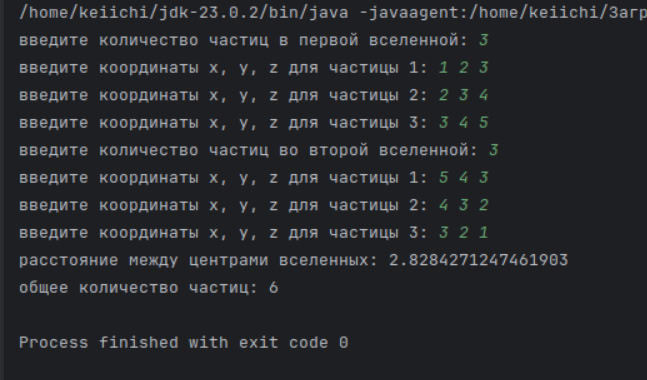
\includegraphics[width=0.8\textwidth]{img1}
\caption{Результат}
\label{fig:img1}
\end{figure}

\end{document}
